\documentclass[12pt,oneside,a4paper]{report}
% Codificação, fonte e idioma
\usepackage[utf8]{inputenc}      % Codificação UTF-8
\usepackage[T1]{fontenc}         % Fonte com suporte a acentuação
\usepackage[portuguese]{babel}   % Hifenização e termos em português

% Fonte (Times New Roman equivalente para pdfLaTeX)
\usepackage{newtxtext}           % Fonte parecida com Times New Roman

% Tipografia
\usepackage{microtype}           % Melhora a justificação
\usepackage{setspace}            % Controle de espaçamento entre linhas
\usepackage{ragged2e}            % Comando \justifying
\onehalfspacing                  % Espaçamento 1,5 entre linhas

% Layout e margens
\usepackage{geometry}
\geometry{
  top=3cm,
  bottom=2cm,
  left=3cm,
  right=2cm
}

% Títulos e espaçamento de capítulos
\usepackage{titlesec}
\titleformat{\chapter}[hang]{\normalfont\Huge\bfseries}{\thechapter}{2em}{}
\titlespacing*{\chapter}{0pt}{0pt}{1.5em}

% Controle de parágrafos
\setlength{\parindent}{1.5cm} % Recuo de parágrafo
\setlength{\parskip}{0pt}     % Sem espaço extra entre parágrafos

% Figuras, tabelas e gráficos
\usepackage{graphicx}
\usepackage{float}
\usepackage{caption}
\usepackage[font=small]{caption}
\usepackage{subcaption}
\usepackage{multirow}
\usepackage{adjustbox}
\DeclareGraphicsExtensions{.png,.jpg,.pdf}

% Tabelas coloridas
\usepackage[table]{xcolor}

% Cores personalizadas
\definecolor{color_200_200_200}{RGB}{200,200,200}
\definecolor{pastelBlue}{RGB}{135, 206, 250}
\definecolor{pastelOrange}{RGB}{255, 178, 102}
\definecolor{pastelRed}{RGB}{240, 128, 128}
\definecolor{pastelGreen}{RGB}{144, 238, 144}
\definecolor{blue}{RGB}{41,5,195}
\definecolor{blue2}{RGB}{41,5,155}
\usepackage{pdfpages}

% Hiperlinks
\usepackage{hyperref}
\hypersetup{
    colorlinks=true,
    linkcolor=blue,
    citecolor=blue2,
    urlcolor=blue,
    filecolor=magenta,
    breaklinks=true
}
\Urlmuskip=0mu plus 1mu % Melhor quebra de links longos

\usepackage[backend=biber, style=abnt]{biblatex} % Estilo ABNT
\renewcommand*{\mkbibnamefamily}[1]{#1} % Remove caixa alta dos sobrenomes nas citações

\addbibresource{bib.bib} % seu arquivo bib






\usepackage{csquotes}



% Estilo da bibliografia
\renewcommand*{\bibfont}{\small\justifying\singlespacing}

% Código fonte
\usepackage{minted} % Lembrar de compilar com --shell-escape

% Outros utilitários
\usepackage{lastpage}
\usepackage{indentfirst}
\usepackage{pifont}
\usepackage{amsmath}
\usepackage{amssymb,amsfonts,amsthm}
\usepackage{etoolbox}
\usepackage{xstring}
\usepackage{hyphenat}
\usepackage{changepage}  % Para recuos
\usepackage{chngcntr}    % Para controlar contadores

% Ajuste na numeração das figuras
\counterwithout{figure}{chapter}
\counterwithout{table}{chapter}
\counterwithout{equation}{chapter} 
\renewcommand{\thesection}{\arabic{section}}
\renewcommand{\thesubsection}{\thesection.\arabic{subsection}}
\setcounter{secnumdepth}{2}
\usepackage{tabularx}
\usepackage{chngcntr}
\counterwithout{footnote}{chapter}


\usepackage[acronym,toc,nonumberlist]{glossaries}
\makeglossaries

\newglossaryentry{termo1}{
    name=Musicoterapia,
    description={Uso da música para promover saúde e bem-estar}
}

\newglossaryentry{midi}{
    name=MIDI,
    description={Musical Instrument Digital Interface, protocolo para comunicação entre instrumentos musicais eletrônicos}
}

 % aqui só definindo os termos do glossário

\usepackage{hyperref}
\usepackage{glossaries}


% Códigos
\renewcommand{\listingscaption}{Código}
\renewcommand{\listoflistingscaption}{Lista de Códigos}

\usepackage{changepage} % para o adjustwidth

\renewenvironment{quote}
  {\begin{adjustwidth}{5cm}{0cm}\fontsize{10}{12}\selectfont}
  {\end{adjustwidth}}

% Seções centralizadas personalizadas (se necessário)
\newcommand{\centersection}[1]{
    \begin{center}
        \textbf{\large #1}
    \end{center}
}
 % arquivo com configurações e imports.
\graphicspath{{arquivos/figuras/}}

% Incluir capa com metadados contidos em "dados.tex"
% Metadados da Tese %
\newcommand{\titulo}{Título do seu trabalho }
\newcommand{\autor}{Nome do doutorando}
\newcommand{\instituicao}{Universidade Federal de Minas Gerais}
\newcommand{\centro}{Escola de Música}
\newcommand{\programa}{Programa de Pós-Graduação em Música}
\newcommand{\linhadepesquisa}{Linha de Pesquisa}

\newcommand{\orientador}{Orientador}
\newcommand{\coorientador}{Coorientador}


 

% Banca %
\newcommand{\membroInterno}{Membro interno da banca}
\newcommand{\membroExterno}{Membro externo da banca 1}
\newcommand{\membroExternodois}{Membro externo da banca 2}

% Instituição do Membro Externo
\newcommand{\instituicaoInterno}{Filiação membro interno }
\newcommand{\instituicaoExterno}{Filiação membro externo 1}
\newcommand{\instituicaoExternodois}{Filiação membro externo 2}

% Cidade onde ocorreu a defesa
\newcommand{\cidade}{Belo Horizonte}
% Estado onde Aconteceu a defesa
\newcommand{\estado}{MG}
% Mês da defesa
\newcommand{\mes}{Mês da defesa}
% Dia da defesa
\newcommand{\dia}{Dia da defesa}
% Ano da defesa
\newcommand{\ano}{Ano da defesa}


% Definindo os metadados do PDF
\hypersetup{
    pdftitle={\titulo},
    pdfauthor={\autor},
    pdfsubject={Tese de Doutorado em Música. Univesidade Federal de Minas Gerais},
    pdfkeywords={Palavra chave, Palavra chave, Palavra chave}}


\begin{document}

%Incluir capa
\begin{center}
    \textbf{\instituicao}\\
    \textbf{\centro}\\
    \textbf{\programa}


    \vspace{4.5cm}
\autor\

    \begin{center}

    \vspace*{\fill} % Ajusta o espaço antes do título (aumenta ou diminui conforme necessário)
   \textbf{\titulo}
    \vspace*{\fill} % Ajusta o espaço depois do título
    \end{center}

    \vfill
    \cidade\ \\
    \ano\
\end{center}
\thispagestyle{empty} % Remove a numeração desta página
\newpage


\begin{center}
\autor\
\end{center}
\vspace{4.5cm}	

\begin{center}	
\textbf{\titulo}
\end{center}



\begin{center}
    \vspace*{\fill} % Ajusta o espaço antes do título (aumenta ou diminui conforme necessário)
    \hspace*{\fill} % Empurra o texto para a direita
    \parbox{10cm} % Ajuste a largura da \parbox conforme necessário para o tamanho do texto
    {\noindent
    Tese apresentada ao Programa de Pós-Graduação em Música, da \instituicao, como requisito parcial à obtenção do título de Doutor em Música.

    \par Linha de Pesquisa: \linhadepesquisa

    \vspace{0.5cm}
    \par Orientador: \orientador{}
    \par Coorientador: \coorientador{}
    }
    \vfill
    \vspace*{\fill} % Ajusta o espaço depois do título
\end{center}


\begin{center}
\cidade\ \\
\ano\
\end{center}

\thispagestyle{empty} % Remove a numeração desta página

% Ficha Catalográfica - TROQUE PELA SUA
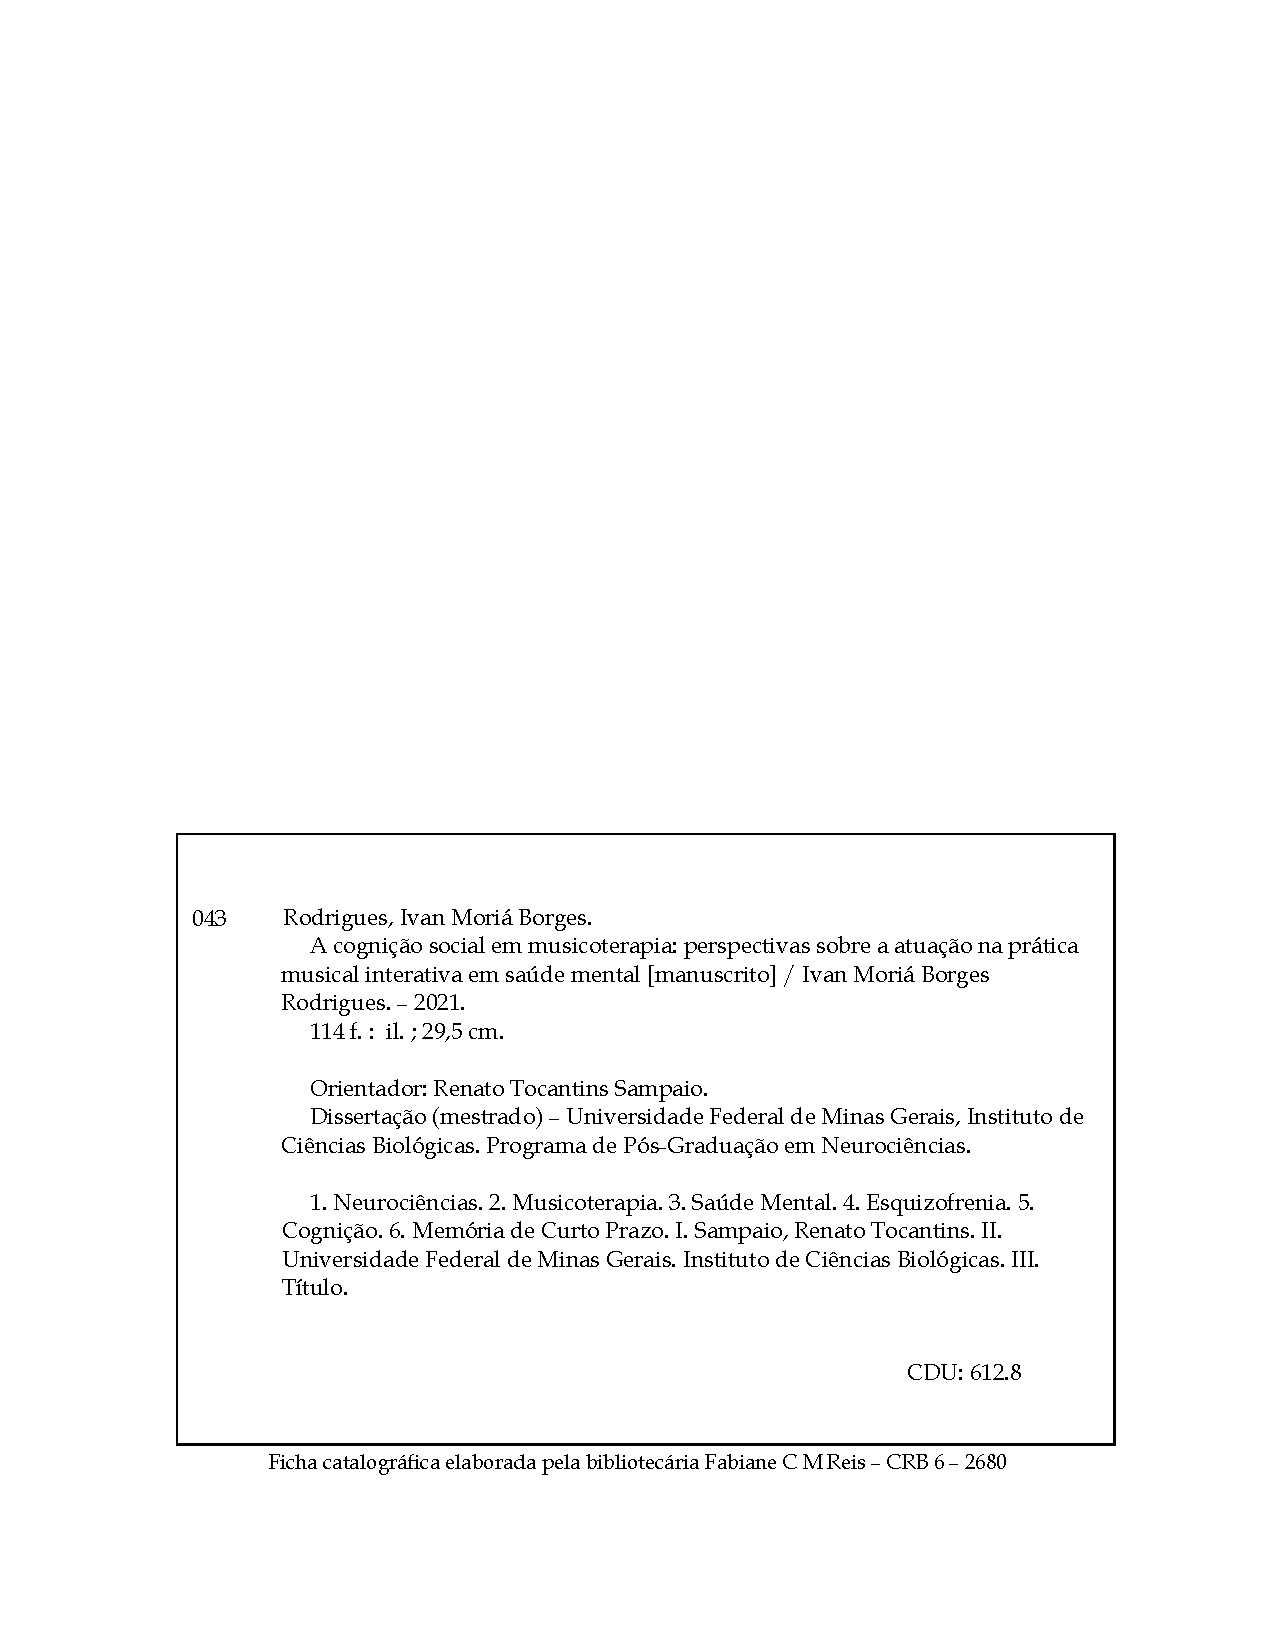
\includepdf{arquivos/pre-texto/Ficha_Catalografica.pdf}

% -------------------------------------------------
% ELEMENTOS PRÉ-Textuais
% -------------------------------------------------

% Folha de aprovação (comente a linha que nao vai utilizar com %)
%Pode fazer manual utilizando o aprovacao.tex

\begin{figure}[h]
    \vspace{-2cm}
    \centering  
    
\includegraphics[scale=0.5]{arquivos/pre-texto/Logo_UFMG.png}\label{fig:logo}
\end{figure}

    \vspace{-1cm}
\begin{center}
    \vspace{0.5cm}
    \textsc{\instituicao}\\
    \textsc{\centro}\\
    \textsc{Programa de Pós-Graduação em Música}
\end{center}

\noindent
Defesa de doutorado de \textbf{\autor}, intitulada \textbf{\titulo} orientado pelo \textbf{Prof.\ Dr.\ \orientador} e coorientado pelo \textbf{Prof.\ Dr.\ \coorientador}, apresentada à banca examinadora designada pelo Colegiado do Programa de Pós-Graduação em Música da UFMG, em \dia\ de \mes\ de \ano. Os membros da Banca Examinadora consideram o candidato: Aprovado.

\begin{center}
    \textbf{BANCA EXAMINADORA}\\

    \vspace{1cm}
    
    \rule{8cm}{0.5pt}\\
    \textbf{Prof.\ Dr.\ \orientador} (Orientador)\\
    \instituicao\ 
    
     \vspace{1cm}
    
    \rule{8cm}{0.5pt}\\
    \textbf{Prof.\ Dr.\ \coorientador} (Coorientador)\\
    \instituicao\ 
    
     \vspace{1cm}
    
    \rule{8cm}{0.5pt}\\
    \textbf{Profa.\ Dra.\ \membroExterno}\\
    \instituicaoExterno
    
     \vspace{1cm}
    
    \rule{8cm}{0.5pt}\\
    \textbf{Prof.\ Dr.\ \membroExternodois}\\
    \instituicaoExternodois
    
     \vspace{1cm}
         
    \rule{8cm}{0.5pt}\\
    \textbf{Prof.\ Dr.\ \membroInterno}\\
    \instituicaoInterno\ 
\end{center}




\vfill




\begin{center}

	\cidade\ \\
     \ano\
\end{center}

% \pagestyle{plain}
% \pagenumbering{roman}
\thispagestyle{empty} % Remove a numeração desta página

%\setcounter{page}{3} %Escolhe-se o estilo de numeração da página.
\newpage




%pode adicionar um pdf caso necessário
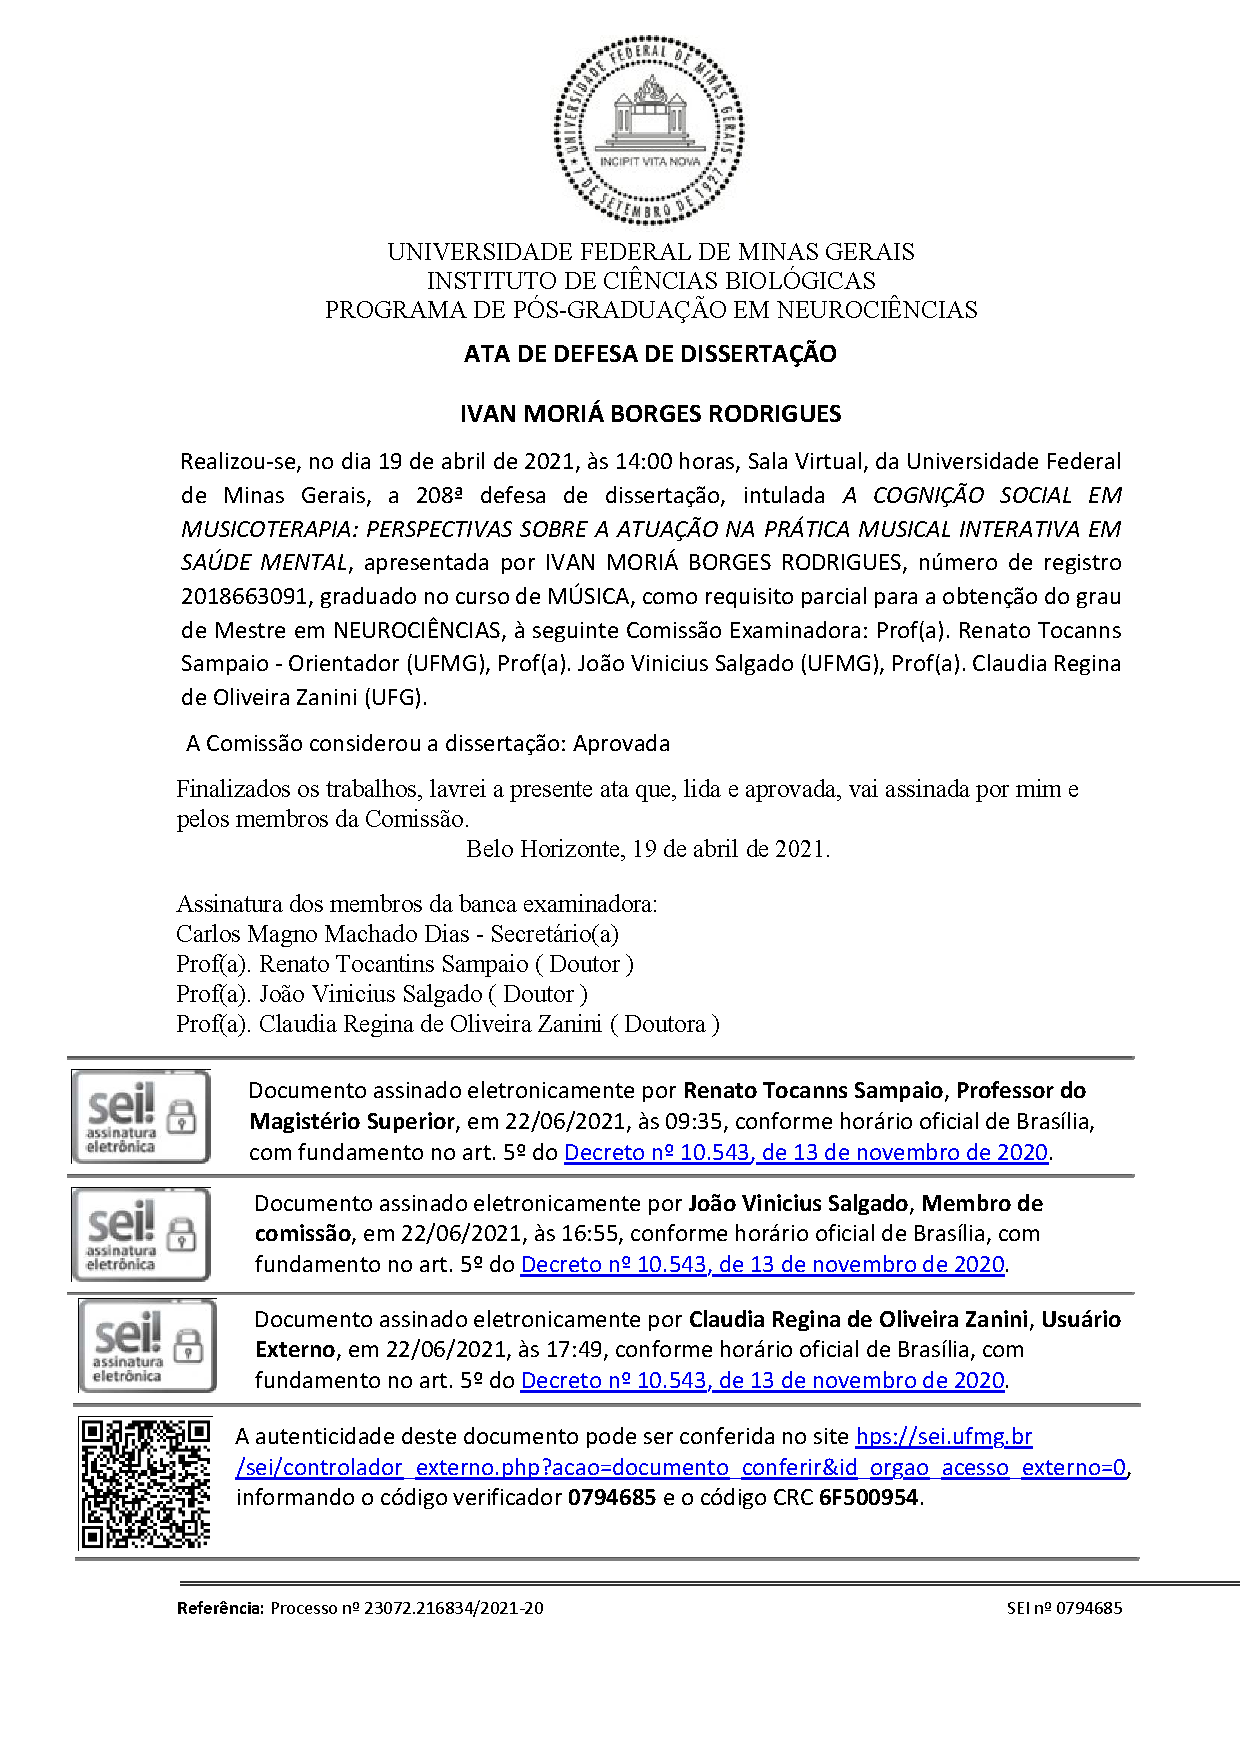
\includepdf{arquivos/pre-texto/aprovacao.pdf}


% Dedicatória
\null\
\vfill

\hfill \parbox{4.0cm} {\noindent \textit{Sua dedicatória. }}





\thispagestyle{empty} % Remove a numeração desta página

\newpage


% Agradecimentos

\centersection{AGRADECIMENTOS}

\begin{flushleft}  % Alinhamento justificado à esquerda
\text{Texto de agradecimentos.} \\
\text{Texto de agradecimentos.} \\
\text{Texto de agradecimentos.} \\
\end{flushleft}

\vspace*{\fill}  % Preenche o espaço vertical restante


\pagenumbering{roman}  % Define a numeração romana
\setcounter{page}{1}  % Começa a numeração romana a partir de 1

\newpage


% Epígrafe
\null\
\vfill

\hfill \parbox{9.0cm} {\noindent Epígrafe. Epígrafe. Epígrafe. Epígrafe. Epígrafe. 


\vspace{0.5cm}

\noindent Autor da Epígrafe. }
\pagenumbering{roman}
\setcounter{page}{2}  % Defini o número da página, altere assim se necessário nas outras páginas.


% Resumo

\centersection{RESUMO} 

Resumo aqui.


\textbf{Palavras-chave}: Palavra. Palavra. Palavra.

\pagenumbering{roman}
\setcounter{page}{3}  % Começa a numeração romana a partir de 1


\newpage



% Abstract

\centersection{ABSTRACT} 


Abstract here.


   
     \textbf{Keywords}: Keyword.





     \pagenumbering{roman}
     \setcounter{page}{4}  

  \newpage

%Adicione comentario caso necessario para remover Lista de Figuras e Tabela etc do Sumário

% Lista de Figuras e Tabelas
\addcontentsline{toc}{section}{Lista de Figuras} 
\listoffigures % Gera a lista de figuras
\newpage % Nova página para separar o conteúdo

\addcontentsline{toc}{section}{Lista de Tabelas} 
\listoftables % Gera a lista de tabelas
\newpage % Nova página para separar o conteúdo

% Lista de Siglas
%Lista de Símbolos
% Lista de códigos

\addcontentsline{toc}{section}{Lista de Códigos} 
\listoflistings\newpage

% ------------------------------------
% SUMÁRIO
% ------------------------------------
\pdfbookmark[0]{\contentsname}{toc}
\tableofcontents % Isso lista o Conteúdo


%------------------------------------------------
% CAPÍTULOS
%-------------------------------------------------
\cleardoublepage
\pagenumbering{arabic} % redefine o estilo de numeração (números arábicos)
\setcounter{page}{1}   % reinicia contagem

\setlength{\parskip}{1.5pt}

\chapter[Introdução]{Introdução}

\section{Introdução \LaTeX}
Você pode querer ter um glossário. Para isso, existe o glossario.tex, um arquivo que você lista todos os que você adicionar. No final do texto eles aparecerão automaticamente. Crie seu glossário e sempre os referencie assim: "Este trabalho aborda a \gls{termo1} e o uso do protocolo \gls{midi}".


Organize seu arquivo \texttt{bib.bib}\footnote{Arquivo BibTeX, deve ser criada uma referência individual e preenchidos os campos. Identifique o tipo entre \texttt{@article}, \texttt{@book}, \texttt{@inproceedings}, etc. Você cria um nome dentro das chaves, por exemplo \texttt{@article\{referencia\}}, e no texto, cita essa referência com \cite{referencia}}. \\ 
Texto com citações: o autor e ano completos entre parênteses cita-se com \cite{article}, somente o ano da referência entre parênteses cita-se com \citeyear{capitulo}. Para citar vários, utilize \parencite{book, congresso, tese, site, manual, relatoriotecnico, naopublicado}.


\vspace{1.5em} %espaço forçado


\begin{quote}
    Citação identada em 5cm. Você pode mudar dentro do arquivo con.tex. Todas as modificações estruturais do arquivo são modificadas separadamente dentro desta configuração. Esse layout define todas os capítulos em diferentes arquivos, separando em blocos e facilitando a edição de forma modular. \cite[p. 00-00]{capitulo}.
\end{quote}

Aqui está uma frase com uma nota de rodapé.\footnote{Este é o texto da nota de rodapé.}



\subsection{Listas}
Enumere listas assim:
\begin{enumerate}
    \item Item 1
    \item Item 2
\end{enumerate}


\subsection{Tabelas}
Crie tabelas desta maneira:


\begin{table}[h!]
    \centering
  
    \label{tab:nometabela}
    \begin{tabular}{|l|p{10cm}|}
    \hline
    \textbf{Parâmetro} & \textbf{Definição} \\ \hline
    \textbf{Título 1}     & Conteúdo \\ \hline
  
    \textbf{Título 2}     & Conteúdo \\ \hline

    \end{tabular}
    \caption{Legenda da tabela 1.}
    \end{table}

Adicione mais linhas ou colunas copiando o conteúdo e adicionando \textbf{\&} para cada nova coluna, desta maneira: 

\begin{table}[h!]
    \centering
   
    \label{tab:nometabela2}
  \begin{tabular}{|l|p{3cm}|p{3cm}|p{3cm}|}

    \hline
    \textbf{Parâmetro} & \textbf{Definição 1} & \textbf{Definição 2} & \textbf{Definição 3} \\ \hline
    \textbf{Título 1}  & Conteúdo            & Conteúdo            & Conteúdo            \\ \hline
    \textbf{Título 2}  & Conteúdo            & Conteúdo            & Conteúdo            \\ \hline

    \textbf{Título 3}  & Conteúdo            & Conteúdo            & Conteúdo            \\ \hline

    
    \end{tabular}
     \caption{Legenda da tabela 2.}
\end{table}

\newpage
%preciso colocar isso para nao quebrar a pagina

\subsection{Imagens}
Para incluir imagens, salve dentro da pasta e mude a referência. No item label, você pode referenciar sua figura com \ref{fig1}. Também pode modificar seu tamanho com width:


\begin{figure}[h]
    \centering

\includegraphics[width=0.2\textwidth]{arquivos/pre-texto/Logo_UFMG.png}
    \caption{Legenda da Imagem 1}
    \label{fig1}
\end{figure}



\subsection{Equações}
Incluindo equações, podendo referenciar como Equação  \ref{ioi_eq1}:

\begin{equation}\label{ioi_eq1}
    IoI_i = t_{i+1} - t_i
\end{equation}

Ou direto no texto, desta maneira:


\[
\text{densidade} = \frac{\text{duração}[1:]}{t_{\text{diff}}}
\]

\vspace{1.5em}


\subsection{Códigos}
Você pode citar o código \ref{lst:codigo-python} desta maneira:


\begin{listing}[h!]
    \centering
    \begin{minted}[frame=lines, style=friendly, linenos=true]{python}
    import numpy as np 
    import pandas as pd  
    \end{minted}
    \caption{Exemplo Python 1}
    \label{lst:codigo-python}
    \end{listing}
    

\newpage

\section{Considerações Finais}

Utilize o comando \texttt{\textbackslash newpage} sempre que necessário para controlar a quebra de página.  
Os demais capítulos estão organizados na pasta \texttt{capitulos}, devendo ser editados separadamente.  
O arquivo principal, \texttt{main.tex}, é responsável por compilar todos os componentes e fazer o \LaTeX\ funcionar corretamente.

\noindent O próximo capítulo é Metodologia, localizado no arquivo \texttt{arquivos/metodologia.tex}.


\subsection{Mais exemplos} 

Imagem:
\begin{figure}[h]
    \centering

\includegraphics[width=0.2\textwidth]{arquivos/pre-texto/Logo_UFMG.png}
    \caption{Legenda da Imagem 2}
    \label{fig2}
\end{figure}

Código Python:
\begin{listing}[h!]
    \centering
    \begin{minted}[frame=lines, style=friendly, linenos=true]{python}
    import numpy as np 
    import pandas as pd  
    \end{minted}
    \caption{Exemplo Python 2 }
    \label{lst:codigo-python2}
    \end{listing}

Tabela mais larga:
\begin{table}[h!]
    \centering
    \begin{tabularx}{\textwidth}{|l|X|X|X|}
        \hline
        \textbf{Parâmetro} & \textbf{Definição 1} & \textbf{Definição 2} & \textbf{Definição 3} \\ \hline
        \textbf{Título 1}  & Conteúdo & Conteúdo & Conteúdo \\ \hline
  
    \end{tabularx}
    \caption{Legenda da tabela 3.}
    \label{tab:nometabela3}
\end{table}




A seguir, Metodologia.

\newpage
\setlength{\parskip}{1.5pt}
\chapter[Metodologia]{Metodologia}

Organize sua metodologia. 
Inclua as considerações éticas do trabalho.


\section{Considerações Éticas}
Aprovado pelo COEP...

\section{Público}

Continue sua metodologia. O próximo arquivo será Resultados
\setlength{\parskip}{1.5pt}
\chapter[Resultados]{Resultados}


Apresente aqui os seus resultados. Inclua imagens, tabelas, glossário como \gls{midi}, referências \cite{article}.



Exemplo de imagem: 
\begin{figure}[h]
    \centering

\includegraphics[width=0.2\textwidth]{arquivos/pre-texto/Logo_UFMG.png}
    \caption{Legenda da Imagem 3}
    \label{fig3}
\end{figure}

Enumere listas assim:
\begin{enumerate}
    \item Item 1
    \item Item 2
\end{enumerate}

Tabela mais larga:
\begin{table}[h!]
    \centering
    \begin{tabularx}{\textwidth}{|l|X|X|X|}
        \hline
        \textbf{Parâmetro} & \textbf{Definição 1} & \textbf{Definição 2} & \textbf{Definição 3} \\ \hline
        \textbf{Título 1}  & Conteúdo & Conteúdo & Conteúdo \\ \hline
        \textbf{Título 2}  & Conteúdo & Conteúdo & Conteúdo \\ \hline
        \textbf{Título 3}  & Conteúdo & Conteúdo & Conteúdo \\ \hline
        
    \end{tabularx}
    \caption{Legenda da tabela 3.}
    \label{tab:nometabela3}
\end{table}


\section{Adicionando pdf}
Talvez você possa incluir um PDF de algum artigo que foi resultado da pesquisa. Para isso, utilize essa lógica neste ponto do documento\footnote{Adicione o seu pdf e mude a localização do arquivo.}:

\begin{listing}[h!]
    \centering
    \begin{minted}[frame=lines, style=friendly, linenos=true]{latex}
\includepdf[pages=-]{arquivos/artigo.pdf}
    \end{minted}
    \caption{Exemplo \LaTeX}
    \label{lst:codigo-latex}
\end{listing}


Finalizando este arquivo, o próximo é Discussão.tex.


\setlength{\parskip}{1.5pt}
\chapter[Discussão]{Discussão}

Não apresente mais nenhuma informação aqui\footnote{Inclusive as siglas, todas já devem ter aparecido antes}. Tudo deve ter sido referenciado anteriormente. Faça a discussão do seu trabalho.


\setlength{\parskip}{1.5pt}
\chapter[Conclusão]{Conclusão}


Conclua seu trabalho.
\chapter*{Referências}
\addcontentsline{toc}{chapter}{Referências}
\printbibliography[heading=none]



\cleardoublepage
\phantomsection
\addcontentsline{toc}{chapter}{Glossário}
\printglossary[title=Glossário, style=altlist]



%  ITENS PÓS-TEXTUAIS  %


% Apêndices
%\chapter*{Apêndices}


\chapter*{Anexos}

Os anexos poderão ser colocados aqui ou via pdf, que será incluído na próxima página. 


\includepdf[pages=-]{arquivos/anexos/diretrizes_UFMG}


\end{document}
